\documentclass[12pt, a4paper, reqno]{article}
\usepackage{labs_preamble}

\begin{document}

\import{./}{title.tex}

\newpage
\tableofcontents
\listoftables
\listoffigures

\newpage
\section{Аннотация}

    В данной работе с помощью сцинтилляционного счётчика измеряются линейные коэффициенты ослабления
    потока $\gamma$-лучей в свинце, железе и алюминии. По величине этих коэффициентов определятся
    энергия $\gamma$-квантов.

\section{Теоретические сведения}

    \textbf{Гамма-излучение} - излучение, возникающее при переходе атомных ядер в состояние с
    меньшей энергией.

    При прохождении через вещество пучок $\gamma$-квантов ослабляется по закону, который можно
    записать в двух эквивалентных формах:
    \begin{equation}\label{I_1}
        I = I_0 e^{-\mu l}
    \end{equation}
    \begin{equation}\label{I_2}
        I = I_0 e^{-\mu' \sigma},
    \end{equation}
    где $I$, $I_0$ - интенсивности прошедшего и падающего излучений, $l$ - длина пути, пройденного
    пучком в веществе, $\sigma$ - масса пройденного вещества, приходящаяся на единицу площади,
    $\mu$, $\mu'$ - константы, величина которых зависит от вещества, сквозь которое проходят лучи
    ($[\mu] = \frac{1}{\text{см}}$, $[\mu'] = \frac{\text{см}^2}{\text{г}}$).

    Данное ослабление обусловлено тремя эффектами: фотоэлектрическим поглощением, комптоновским
    рассеянием и генерацией электрон-позитронных пар. При этом коэффициент $\mu$ равен сумме таких
    коэффициентов для этих трёх процессов.

    Рассмотрим случай \textit{хорошей геометрии}, т.е. пучок $\gamma$-лучей предполагается узким и
    тонким. В этом случае комптоновское рассеяние и генерация пар выводят $\gamma$-кванты из пучка.
    Поэтому при прохождении через вещество количество квантов меняется, а их энергия - нет.

    Обозначим через $-dN$ число $\gamma$-квантов, выбывших из пучка на пути $dl$. Вследствие
    \textit{хорошей геометрии} имеем:
    \begin{equation*}
        -dN = \mu N dl,\ \mu = const
    \end{equation*}
    Интрегрированием последнего соотношения получим:
    \begin{equation*}
        N = N_0 e^{-\mu l},
    \end{equation*}
    где $N_0$, $N$ - число $\gamma$-квантов в падающем и прошедшем излучении, соответственно.
    Последняя формула является аналогом формул \eqref{I_1} и \eqref{I_2}. Далее, находим:
    \begin{equation}\label{mu_coeff}
        \boxed{\mu = \frac{1}{l}\ln{\frac{N_0}{N}}}
    \end{equation}

\newpage
\section{Экспериментальная установка}

    Схема установки показана на рисунке \ref{fig:scheme}.
    \begin{figure}[H]
        \centering
        \caption{Схема экспериментальной установки}
        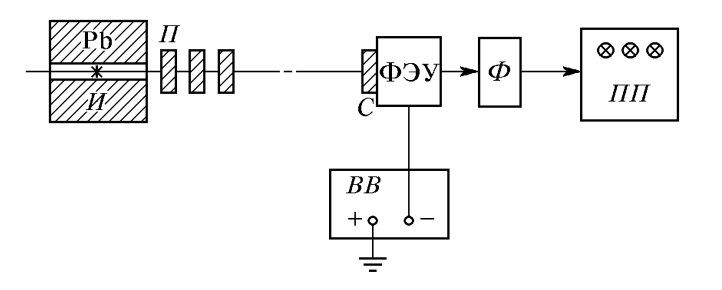
\includegraphics[width = 0.8\textwidth]{scheme.png}
        \label{fig:scheme}
    \end{figure}

    Свинцовые коллиматор выделяет узкий почти параллельный пучок $\gamma$-квантов, проходящий через
    набор поглотителей П и регистрируемый сцинтилляционным счётчиком. Сигналы от счётчика
    усиливаются и регистрируются пересчётным прибором ПП. Высоковольтный выпрямитель ВВ обеспечивает
    питание сцинтилляционного счётчика.

    Для того, чтобы $\gamma$-кванты, провзаимодействовавшие в поглотителе и вернувшиеся в пучок, не
    попали в сцинтилляционный счётчик, его следует распологать на достаточно большом расстоянии от
    источника $\gamma$-квантов.

\section{Измерения и обработка их результатов}

    Каждое измерение числа частиц проводилось в течение 60 секунд.

    Сначала был измерен фон, то есть число зарегистрированных частиц при закрытом коллиматоре.
    Результаты приведены в таблице \ref{table:background}.

    На основании этих измерений найдём среднее значение фона и его дисперсию.
    \begin{equation*}
        \overline{N_{\text{ф}}} = \frac{1}{3}\sum_{i = 1}^{3} N_i \approx 1820; \ \ \
        \sigma_{\text{ф}} = \sqrt{\frac{1}{3 - 1} \sum_{i = 1}^{3}(N_i - \overline{N_{\text{ф}}})^2}
        \approx 82
    \end{equation*}

    Таким образом, для фона имеем:
    \begin{equation*}
        \boxed{N_{\text{ф}} = 1820 \pm 82}
    \end{equation*}

    Далее было проведено измерение числа частиц, прошедших через образец при открытом коллиматоре,
    для разных материалов разной толщины. Последнего удалось добиться путём изменения числа
    поглотителей одинаковой толщины. Результаты измерения толщины одного поглотителя приведены в
    таблице \ref{table:depth}.

    Результаты измерений числа частиц, прошедших через поглотители, приведены в таблицах
    \ref{table:Al}, \ref{table:Fe}, \ref{table:Pb}. Также было измерено число частиц в отсутствие
    поглотителей:
    \begin{equation*}
        \boxed{N_0 = 550204}
    \end{equation*}

    Запишем формулу \eqref{mu_coeff} в альтернативной форме, заодно учитывая наличие фона:
    \begin{equation*}
        \ln{(N - N_{\text{ф}})} = \ln{(N_0 - N_{\text{ф}})} - \mu l
    \end{equation*}
    Из этого выражения видно, что $\mu$ - угловой коэффициент аппроксимирующей прямой на графике
    $(\ln(N - N_{\text{ф}}))(l)$. На основании данных из таблиц построим график \ref{fig:chart}.
    Линейные коэффициенты поглощения $\gamma$-лучей:
    \begin{equation*}
        \boxed{\mu_{Al} = (0.185 \pm 0.002)\ \text{см}^{-1}}
    \end{equation*}
    \begin{equation*}
        \boxed{\mu_{Pb} = (0.74 \pm 0.05)\ \text{см}^{-1}}
    \end{equation*}
    \begin{equation*}
        \boxed{\mu_{Fe} = (0.335 \pm 0.009)\ \text{см}^{-1}}
    \end{equation*}

    Обратимся к таблице V.4 "Линейные коэффициенты поглощения $\gamma$-лучей в различных веществах"\
    из лабника. Опреледим по ней энергии $\gamma$-квантов:
    \begin{equation*}
        \boxed{E_{Al} \approx 0.8\ \text{МэВ}}
    \end{equation*}
    \begin{equation*}
        \boxed{E_{Pb} \approx 1.0\ \text{МэВ}}
    \end{equation*}
    \begin{equation*}
        \boxed{E_{Fe} \approx 2.0\ \text{МэВ}}
    \end{equation*}


\section{Вывод}

    В ходе работы были получены линейные коэффициенты поглощения $\gamma$-лучей. Из этих
    коэффициентов были получены энергии $\gamma$-квантов, которые оказались различными для трёх
    материалов поглотителей. Возможным объяснением такого результата могут служить примеси,
    содержащиеся в поглотителях.

\newpage
\section{Приложения}

    \subsection{Таблицы}

        \begin{table}[H]
            \centering
            \caption{Измерения фона}
            \begin{tabular}{|c|c|}
                \hline
                Номер измерения & Число прошедших частиц \\ \hline\hline
                1               & 1908                   \\ \hline
                2               & 1746                   \\ \hline
                3               & 1807                   \\ \hline
            \end{tabular}
            \label{table:background}
        \end{table}

        \begin{table}[H]
            \centering
            \caption{Толщины поглотителей}
            \begin{tabular}{|c|c|}
                \hline
                Материал & $l_0$, cм \\ \hline\hline
                Алюминий & 1.98      \\ \hline
                Свинец   & 0.42      \\ \hline
                Железо   & 1.01      \\ \hline
            \end{tabular}
            \label{table:depth}
        \end{table}

        \begin{minipage}{0.33\textwidth}
            \centering
            \captionof{table}{Алюминий}
            \begin{tabular}{|c|c|}
                \hline
                Число брусков & N       \\ \hline\hline
                1             & 387597  \\ \hline
                2             & 287608  \\ \hline
                3             & 192787  \\ \hline
                4             & 141892  \\ \hline
                5             & 95683   \\ \hline
                6             & 67870   \\ \hline
                7             & 45874   \\ \hline
                8             & 33481   \\ \hline
                9             & 23257   \\ \hline
                10            & 16317   \\ \hline
            \end{tabular}
            \label{table:Al}
        \end{minipage}
        \begin{minipage}{0.33\textwidth}
            \centering
            \captionof{table}{Свинец}
            \begin{tabular}{|c|c|}
                \hline
                Число брусков & N \\ \hline\hline
                1 & 396703        \\ \hline
                2 & 254763        \\ \hline
                3 & 177644        \\ \hline
                4 & 132110        \\ \hline
                5 & 102483        \\ \hline
                6 & 84341         \\ \hline
            \end{tabular}
            \label{table:Fe}
        \end{minipage}
        \begin{minipage}{0.33\textwidth}
            \centering
            \captionof{table}{Железо}
            \begin{tabular}{|c|c|}
                \hline
                Число брусков & N       \\ \hline\hline
                1             & 365055  \\ \hline
                2             & 250826  \\ \hline
                3             & 166156  \\ \hline
                4             & 114470  \\ \hline
                5             & 77888   \\ \hline
                6             & 53637   \\ \hline
                7             & 39070   \\ \hline
                8             & 28473   \\ \hline
                9             & 22190   \\ \hline
                10            & 16564   \\ \hline
                11            & 14694   \\ \hline
                12            & 10396   \\ \hline
            \end{tabular}
            \label{table:Pb}
        \end{minipage}

\newpage

    \subsection{Графики}

        \begin{figure}[H]
            \centering
            \caption{Зависимость логарифма числа частиц от толщины образца}
            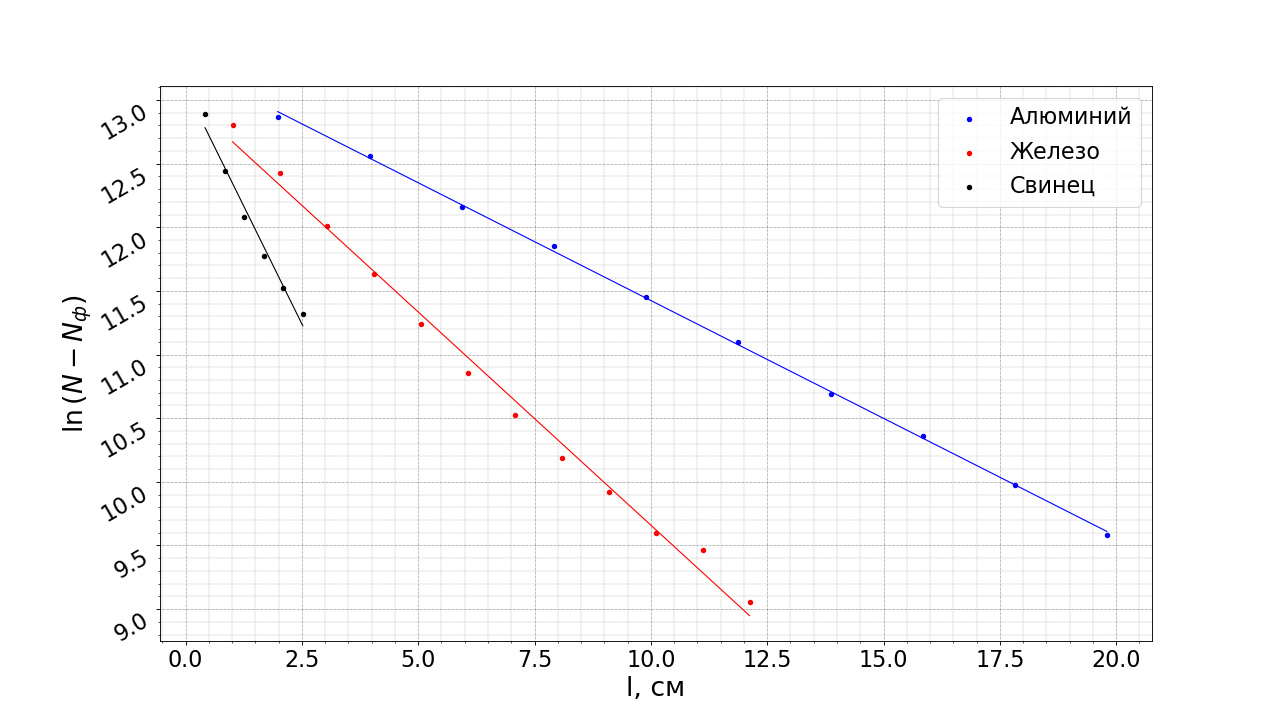
\includegraphics[width = \textwidth]{chart.png}
            \label{fig:chart}
        \end{figure}

\end{document}
